\begin{frame}
  \frametitle{Modello Shigesada-Okubo (1981)}
  \[ n(z,t) \]
  \[ \partial_t n + v \partial_z n = D \partial_z^2 n + (g(z,n) - \mu) n \]
  \[ g(z,n) =  \lambda \frac{I(z,t)}{I(z,t)+h} \]
  \[ I(z,t) = e^{-k_{bg} z - k_{as}\int_0^z n(z,t) } \]

  \begin{columns}
    \column{0.5\textwidth}
    \begin{block}{Condizioni al contorno di no-flux}
      \( v n - D \partial_z n = 0\)
    \end{block}
  \end{columns}
\end{frame}

\begin{frame}
  \frametitle{Modello Huisman (2002)}
  \begin{columns}
    \column{.5\textwidth}
    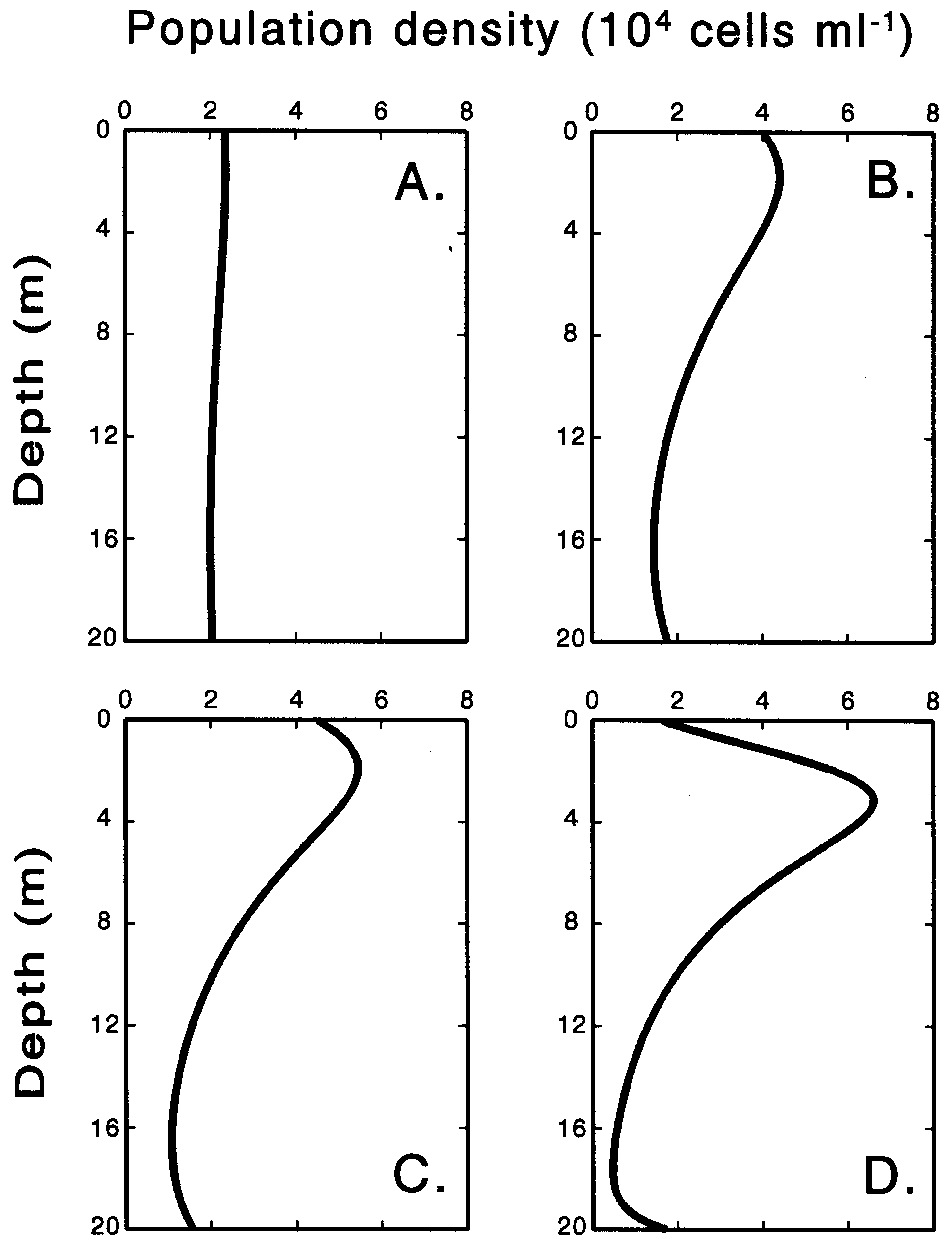
\includegraphics[width=\textwidth]{../img/pl_peak_Huis}

    \column{.5\textwidth}
    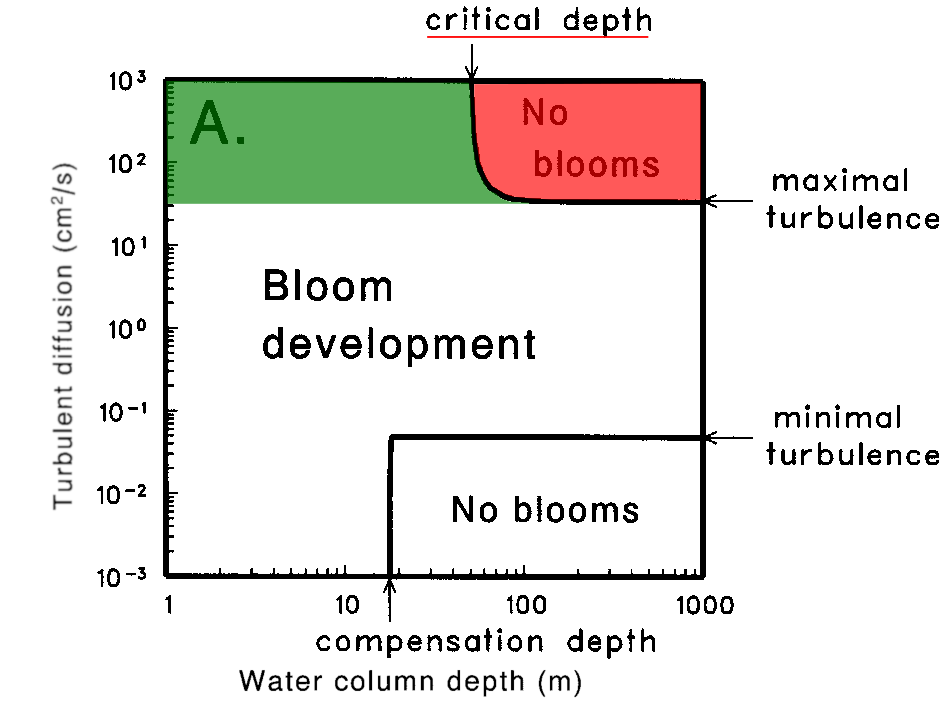
\includegraphics[width=\textwidth]{../img/result_Huis_lowvel}
    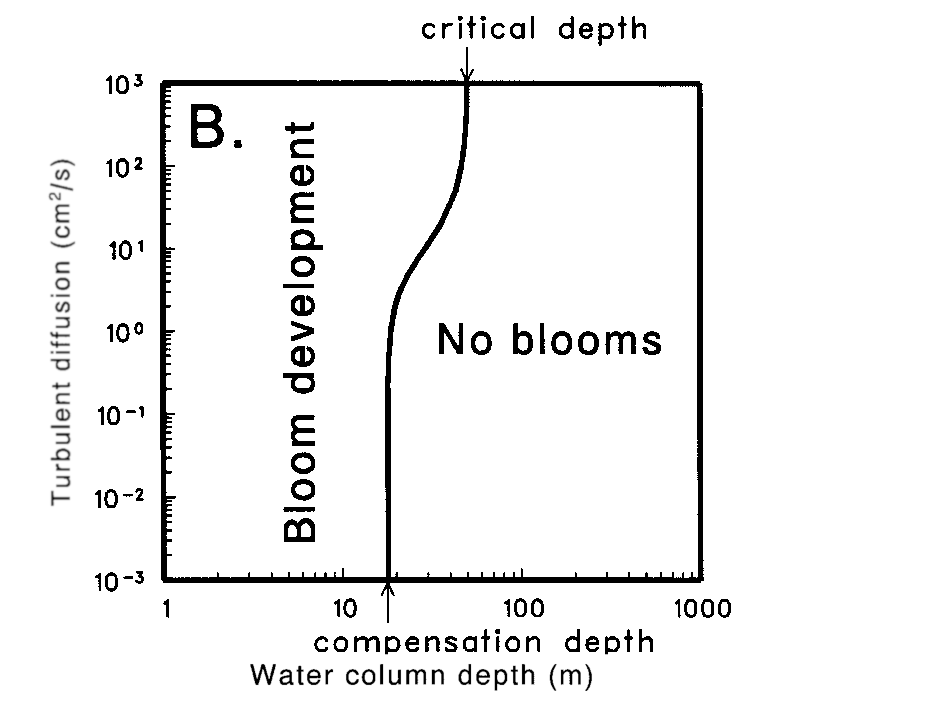
\includegraphics[width=\textwidth]{../img/result_Huis_hivel}

  \end{columns}
\end{frame}
